\section{Referencia de la Clase God\-Zilla}
\label{classGodZilla}\index{GodZilla@{GodZilla}}
{\tt \#include $<$godzilla.h$>$}

Diagrama de colaboraci\'{o}n para God\-Zilla:\begin{figure}[H]
\begin{center}
\leavevmode
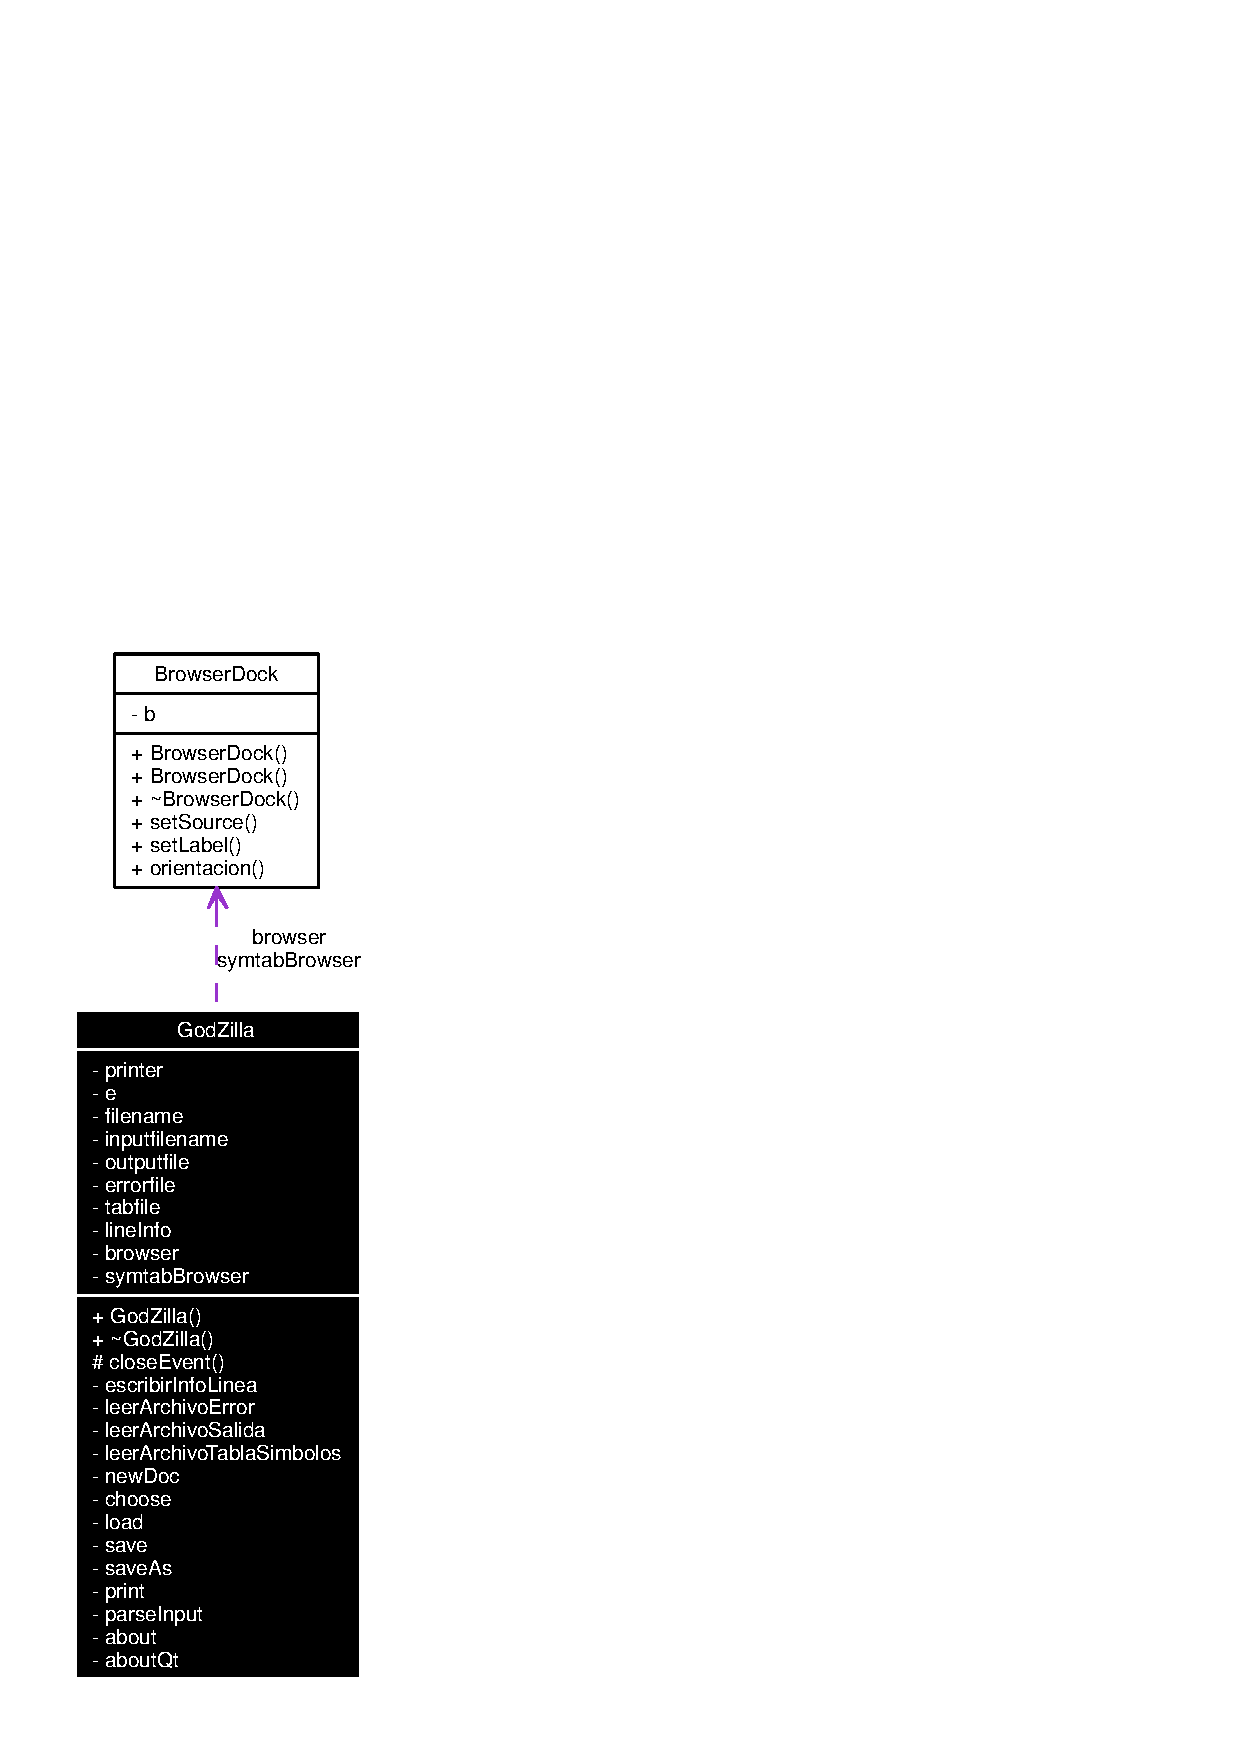
\includegraphics[width=87pt]{classGodZilla__coll__graph}
\end{center}
\end{figure}
\subsection*{M\'{e}todos p\'{u}blicos}
\begin{CompactItemize}
\item 
{\bf God\-Zilla} ()
\item 
{\bf $\sim$God\-Zilla} ()
\end{CompactItemize}
\subsection*{M\'{e}todos protegidos}
\begin{CompactItemize}
\item 
void {\bf close\-Event} (QClose\-Event $\ast$)
\end{CompactItemize}
\subsection*{Slots privados}
\begin{CompactItemize}
\item 
void {\bf escribir\-Info\-Linea} (int row, int col)
\begin{CompactList}\small\item\em slot para escribir linea de archivo al widget line\-Info contenido en la barra de estados \item\end{CompactList}\item 
void {\bf leer\-Archivo\-Error} ()
\begin{CompactList}\small\item\em Abre en el browser el archivo de error. \item\end{CompactList}\item 
void {\bf leer\-Archivo\-Salida} ()
\begin{CompactList}\small\item\em Abre en el browser el archivo de salida. \item\end{CompactList}\item 
void {\bf leer\-Archivo\-Tabla\-Simbolos} ()
\begin{CompactList}\small\item\em Abre en el browser el archivo de tabla de simbolos. \item\end{CompactList}\item 
void {\bf new\-Doc} ()
\item 
void {\bf choose} ()
\item 
void {\bf load} (const QString \&file\-Name)
\item 
void {\bf save} ()
\item 
void {\bf save\-As} ()
\item 
void {\bf print} ()
\begin{CompactList}\small\item\em Llama al modulo de impresion del shell. \item\end{CompactList}\item 
int {\bf parse\-Input} ()
\begin{CompactList}\small\item\em Slot para el boton de analisis del archivo de entrada. \item\end{CompactList}\item 
void {\bf about} ()
\begin{CompactList}\small\item\em Muestra dialogo. \item\end{CompactList}\item 
void {\bf about\-Qt} ()
\end{CompactItemize}
\subsection*{Atributos privados}
\begin{CompactItemize}
\item 
QPrinter $\ast$ {\bf printer}
\item 
QText\-Edit $\ast$ {\bf e}
\item 
QString {\bf filename}
\item 
QString {\bf inputfilename}
\item 
QString {\bf outputfile}
\item 
QString {\bf errorfile}
\item 
QString {\bf tabfile}
\item 
QLabel $\ast$ {\bf line\-Info}
\item 
{\bf Browser\-Dock} $\ast$ {\bf browser}
\item 
{\bf Browser\-Dock} $\ast$ {\bf symtab\-Browser}
\end{CompactItemize}


\subsection{Descripci\'{o}n detallada}




Definici\'{o}n en la l\'{\i}nea 30 del archivo godzilla.h.

\subsection{Documentaci\'{o}n del constructor y destructor}
\index{GodZilla@{God\-Zilla}!GodZilla@{GodZilla}}
\index{GodZilla@{GodZilla}!GodZilla@{God\-Zilla}}
\subsubsection{\setlength{\rightskip}{0pt plus 5cm}God\-Zilla::God\-Zilla ()}\label{classGodZilla_a0}




Definici\'{o}n en la l\'{\i}nea 33 del archivo godzilla.cpp.

Hace referencia a about(), about\-Qt(), browser, choose(), e, escribir\-Info\-Linea(), leer\-Archivo\-Error(), leer\-Archivo\-Salida(), leer\-Archivo\-Tabla\-Simbolos(), line\-Info, new\-Doc(), parse\-Input(), print(), printer, save(), save\-As(), y Browser\-Dock::set\-Label().\index{GodZilla@{God\-Zilla}!~GodZilla@{$\sim$GodZilla}}
\index{~GodZilla@{$\sim$GodZilla}!GodZilla@{God\-Zilla}}
\subsubsection{\setlength{\rightskip}{0pt plus 5cm}God\-Zilla::$\sim$God\-Zilla ()}\label{classGodZilla_a1}




Definici\'{o}n en la l\'{\i}nea 186 del archivo godzilla.cpp.

Hace referencia a printer.

\subsection{Documentaci\'{o}n de las funciones miembro}
\index{GodZilla@{God\-Zilla}!about@{about}}
\index{about@{about}!GodZilla@{God\-Zilla}}
\subsubsection{\setlength{\rightskip}{0pt plus 5cm}void God\-Zilla::about ()\hspace{0.3cm}{\tt  [private, slot]}}\label{classGodZilla_k11}


Muestra dialogo. 



Definici\'{o}n en la l\'{\i}nea 413 del archivo godzilla.cpp.

Referenciado por God\-Zilla().\index{GodZilla@{God\-Zilla}!aboutQt@{aboutQt}}
\index{aboutQt@{aboutQt}!GodZilla@{God\-Zilla}}
\subsubsection{\setlength{\rightskip}{0pt plus 5cm}void God\-Zilla::about\-Qt ()\hspace{0.3cm}{\tt  [private, slot]}}\label{classGodZilla_k12}




Definici\'{o}n en la l\'{\i}nea 422 del archivo godzilla.cpp.

Referenciado por God\-Zilla().\index{GodZilla@{God\-Zilla}!choose@{choose}}
\index{choose@{choose}!GodZilla@{God\-Zilla}}
\subsubsection{\setlength{\rightskip}{0pt plus 5cm}void God\-Zilla::choose ()\hspace{0.3cm}{\tt  [private, slot]}}\label{classGodZilla_k5}




Definici\'{o}n en la l\'{\i}nea 199 del archivo godzilla.cpp.

Hace referencia a load().

Referenciado por God\-Zilla().\index{GodZilla@{God\-Zilla}!closeEvent@{closeEvent}}
\index{closeEvent@{closeEvent}!GodZilla@{God\-Zilla}}
\subsubsection{\setlength{\rightskip}{0pt plus 5cm}void God\-Zilla::close\-Event (QClose\-Event $\ast$)\hspace{0.3cm}{\tt  [protected]}}\label{classGodZilla_b0}




Definici\'{o}n en la l\'{\i}nea 386 del archivo godzilla.cpp.

Hace referencia a e, y save().\index{GodZilla@{God\-Zilla}!escribirInfoLinea@{escribirInfoLinea}}
\index{escribirInfoLinea@{escribirInfoLinea}!GodZilla@{God\-Zilla}}
\subsubsection{\setlength{\rightskip}{0pt plus 5cm}void God\-Zilla::escribir\-Info\-Linea (int {\em row}, int {\em col})\hspace{0.3cm}{\tt  [private, slot]}}\label{classGodZilla_k0}


slot para escribir linea de archivo al widget line\-Info contenido en la barra de estados 



Definici\'{o}n en la l\'{\i}nea 320 del archivo godzilla.cpp.

Hace referencia a line\-Info.

Referenciado por God\-Zilla().\index{GodZilla@{God\-Zilla}!leerArchivoError@{leerArchivoError}}
\index{leerArchivoError@{leerArchivoError}!GodZilla@{God\-Zilla}}
\subsubsection{\setlength{\rightskip}{0pt plus 5cm}void God\-Zilla::leer\-Archivo\-Error ()\hspace{0.3cm}{\tt  [private, slot]}}\label{classGodZilla_k1}


Abre en el browser el archivo de error. 



Definici\'{o}n en la l\'{\i}nea 324 del archivo godzilla.cpp.

Hace referencia a browser, errorfile, y Browser\-Dock::set\-Source().

Referenciado por God\-Zilla().\index{GodZilla@{God\-Zilla}!leerArchivoSalida@{leerArchivoSalida}}
\index{leerArchivoSalida@{leerArchivoSalida}!GodZilla@{God\-Zilla}}
\subsubsection{\setlength{\rightskip}{0pt plus 5cm}void God\-Zilla::leer\-Archivo\-Salida ()\hspace{0.3cm}{\tt  [private, slot]}}\label{classGodZilla_k2}


Abre en el browser el archivo de salida. 



Definici\'{o}n en la l\'{\i}nea 338 del archivo godzilla.cpp.

Hace referencia a browser, outputfile, y Browser\-Dock::set\-Source().

Referenciado por God\-Zilla().\index{GodZilla@{God\-Zilla}!leerArchivoTablaSimbolos@{leerArchivoTablaSimbolos}}
\index{leerArchivoTablaSimbolos@{leerArchivoTablaSimbolos}!GodZilla@{God\-Zilla}}
\subsubsection{\setlength{\rightskip}{0pt plus 5cm}void God\-Zilla::leer\-Archivo\-Tabla\-Simbolos ()\hspace{0.3cm}{\tt  [private, slot]}}\label{classGodZilla_k3}


Abre en el browser el archivo de tabla de simbolos. 



Definici\'{o}n en la l\'{\i}nea 331 del archivo godzilla.cpp.

Hace referencia a browser, outputfile, y Browser\-Dock::set\-Source().

Referenciado por God\-Zilla().\index{GodZilla@{God\-Zilla}!load@{load}}
\index{load@{load}!GodZilla@{God\-Zilla}}
\subsubsection{\setlength{\rightskip}{0pt plus 5cm}void God\-Zilla::load (const QString \& {\em file\-Name})\hspace{0.3cm}{\tt  [private, slot]}}\label{classGodZilla_k6}




Definici\'{o}n en la l\'{\i}nea 210 del archivo godzilla.cpp.

Hace referencia a e, filename, y inputfilename.

Referenciado por choose().\index{GodZilla@{God\-Zilla}!newDoc@{newDoc}}
\index{newDoc@{newDoc}!GodZilla@{God\-Zilla}}
\subsubsection{\setlength{\rightskip}{0pt plus 5cm}void God\-Zilla::new\-Doc ()\hspace{0.3cm}{\tt  [private, slot]}}\label{classGodZilla_k4}




Definici\'{o}n en la l\'{\i}nea 192 del archivo godzilla.cpp.

Referenciado por God\-Zilla().\index{GodZilla@{God\-Zilla}!parseInput@{parseInput}}
\index{parseInput@{parseInput}!GodZilla@{God\-Zilla}}
\subsubsection{\setlength{\rightskip}{0pt plus 5cm}int God\-Zilla::parse\-Input ()\hspace{0.3cm}{\tt  [private, slot]}}\label{classGodZilla_k10}


Slot para el boton de analisis del archivo de entrada. 



Definici\'{o}n en la l\'{\i}nea 273 del archivo godzilla.cpp.

Hace referencia a browser, errorfile, generar\-Salida\-Error(), inputfilename, inputparse(), outputfile, Browser\-Dock::set\-Source(), y tabfile.

Referenciado por God\-Zilla().\index{GodZilla@{God\-Zilla}!print@{print}}
\index{print@{print}!GodZilla@{God\-Zilla}}
\subsubsection{\setlength{\rightskip}{0pt plus 5cm}void God\-Zilla::print ()\hspace{0.3cm}{\tt  [private, slot]}}\label{classGodZilla_k9}


Llama al modulo de impresion del shell. 



Definici\'{o}n en la l\'{\i}nea 347 del archivo godzilla.cpp.

Hace referencia a e, y printer.

Referenciado por God\-Zilla().\index{GodZilla@{God\-Zilla}!save@{save}}
\index{save@{save}!GodZilla@{God\-Zilla}}
\subsubsection{\setlength{\rightskip}{0pt plus 5cm}void God\-Zilla::save ()\hspace{0.3cm}{\tt  [private, slot]}}\label{classGodZilla_k7}




Definici\'{o}n en la l\'{\i}nea 228 del archivo godzilla.cpp.

Hace referencia a e, filename, inputfilename, y save\-As().

Referenciado por close\-Event(), God\-Zilla(), y save\-As().\index{GodZilla@{God\-Zilla}!saveAs@{saveAs}}
\index{saveAs@{saveAs}!GodZilla@{God\-Zilla}}
\subsubsection{\setlength{\rightskip}{0pt plus 5cm}void God\-Zilla::save\-As ()\hspace{0.3cm}{\tt  [private, slot]}}\label{classGodZilla_k8}




Definici\'{o}n en la l\'{\i}nea 255 del archivo godzilla.cpp.

Hace referencia a filename, inputfilename, y save().

Referenciado por God\-Zilla(), y save().

\subsection{Documentaci\'{o}n de los datos miembro}
\index{GodZilla@{God\-Zilla}!browser@{browser}}
\index{browser@{browser}!GodZilla@{God\-Zilla}}
\subsubsection{\setlength{\rightskip}{0pt plus 5cm}{\bf Browser\-Dock}$\ast$ {\bf God\-Zilla::browser}\hspace{0.3cm}{\tt  [private]}}\label{classGodZilla_r8}




Definici\'{o}n en la l\'{\i}nea 68 del archivo godzilla.h.

Referenciado por God\-Zilla(), leer\-Archivo\-Error(), leer\-Archivo\-Salida(), leer\-Archivo\-Tabla\-Simbolos(), y parse\-Input().\index{GodZilla@{God\-Zilla}!e@{e}}
\index{e@{e}!GodZilla@{God\-Zilla}}
\subsubsection{\setlength{\rightskip}{0pt plus 5cm}QText\-Edit$\ast$ {\bf God\-Zilla::e}\hspace{0.3cm}{\tt  [private]}}\label{classGodZilla_r1}




Definici\'{o}n en la l\'{\i}nea 61 del archivo godzilla.h.

Referenciado por close\-Event(), God\-Zilla(), load(), print(), y save().\index{GodZilla@{God\-Zilla}!errorfile@{errorfile}}
\index{errorfile@{errorfile}!GodZilla@{God\-Zilla}}
\subsubsection{\setlength{\rightskip}{0pt plus 5cm}QString {\bf God\-Zilla::errorfile}\hspace{0.3cm}{\tt  [private]}}\label{classGodZilla_r5}




Definici\'{o}n en la l\'{\i}nea 65 del archivo godzilla.h.

Referenciado por leer\-Archivo\-Error(), y parse\-Input().\index{GodZilla@{God\-Zilla}!filename@{filename}}
\index{filename@{filename}!GodZilla@{God\-Zilla}}
\subsubsection{\setlength{\rightskip}{0pt plus 5cm}QString {\bf God\-Zilla::filename}\hspace{0.3cm}{\tt  [private]}}\label{classGodZilla_r2}




Definici\'{o}n en la l\'{\i}nea 62 del archivo godzilla.h.

Referenciado por load(), save(), y save\-As().\index{GodZilla@{God\-Zilla}!inputfilename@{inputfilename}}
\index{inputfilename@{inputfilename}!GodZilla@{God\-Zilla}}
\subsubsection{\setlength{\rightskip}{0pt plus 5cm}QString {\bf God\-Zilla::inputfilename}\hspace{0.3cm}{\tt  [private]}}\label{classGodZilla_r3}




Definici\'{o}n en la l\'{\i}nea 63 del archivo godzilla.h.

Referenciado por load(), parse\-Input(), save(), y save\-As().\index{GodZilla@{God\-Zilla}!lineInfo@{lineInfo}}
\index{lineInfo@{lineInfo}!GodZilla@{God\-Zilla}}
\subsubsection{\setlength{\rightskip}{0pt plus 5cm}QLabel$\ast$ {\bf God\-Zilla::line\-Info}\hspace{0.3cm}{\tt  [private]}}\label{classGodZilla_r7}




Definici\'{o}n en la l\'{\i}nea 67 del archivo godzilla.h.

Referenciado por escribir\-Info\-Linea(), y God\-Zilla().\index{GodZilla@{God\-Zilla}!outputfile@{outputfile}}
\index{outputfile@{outputfile}!GodZilla@{God\-Zilla}}
\subsubsection{\setlength{\rightskip}{0pt plus 5cm}QString {\bf God\-Zilla::outputfile}\hspace{0.3cm}{\tt  [private]}}\label{classGodZilla_r4}




Definici\'{o}n en la l\'{\i}nea 64 del archivo godzilla.h.

Referenciado por leer\-Archivo\-Salida(), leer\-Archivo\-Tabla\-Simbolos(), y parse\-Input().\index{GodZilla@{God\-Zilla}!printer@{printer}}
\index{printer@{printer}!GodZilla@{God\-Zilla}}
\subsubsection{\setlength{\rightskip}{0pt plus 5cm}QPrinter$\ast$ {\bf God\-Zilla::printer}\hspace{0.3cm}{\tt  [private]}}\label{classGodZilla_r0}




Definici\'{o}n en la l\'{\i}nea 60 del archivo godzilla.h.

Referenciado por God\-Zilla(), print(), y $\sim$God\-Zilla().\index{GodZilla@{God\-Zilla}!symtabBrowser@{symtabBrowser}}
\index{symtabBrowser@{symtabBrowser}!GodZilla@{God\-Zilla}}
\subsubsection{\setlength{\rightskip}{0pt plus 5cm}{\bf Browser\-Dock}$\ast$ {\bf God\-Zilla::symtab\-Browser}\hspace{0.3cm}{\tt  [private]}}\label{classGodZilla_r9}




Definici\'{o}n en la l\'{\i}nea 69 del archivo godzilla.h.\index{GodZilla@{God\-Zilla}!tabfile@{tabfile}}
\index{tabfile@{tabfile}!GodZilla@{God\-Zilla}}
\subsubsection{\setlength{\rightskip}{0pt plus 5cm}QString {\bf God\-Zilla::tabfile}\hspace{0.3cm}{\tt  [private]}}\label{classGodZilla_r6}




Definici\'{o}n en la l\'{\i}nea 66 del archivo godzilla.h.

Referenciado por parse\-Input().

La documentaci\'{o}n para esta clase fu\'{e} generada a partir de los siguientes archivos:\begin{CompactItemize}
\item 
/media/docs/progra/c++/compiladores1/proy2/godzilla/src/{\bf godzilla.h}\item 
/media/docs/progra/c++/compiladores1/proy2/godzilla/src/{\bf godzilla.cpp}\end{CompactItemize}
